\section{The original results (superseded)}\label{app:original}
The first version of this paper reported the experiments below, run on the original simulator. An independent review found that
this simulator (i) drew the initialisation, the data order and all device randomness from one shared random stream, so that two
arms of the same seed did not share their initial weights or their data order; (ii) moved the TTv2 and c-TTv2 accumulator
straight to its symmetry point while charging 62 pulses it did not apply; and (iii) copied the AIHWKIT preset fields into a
model with different bounds and no slope spread. The results are kept here unchanged, as preliminary results of that
simulator; the revised experiments of Sections~\ref{sec:main}--\ref{sec:spec} replace them. The diagnostic of
Appendix~\ref{app:revision} measures how much each repair moves them.

The original headline readings were: plain SGD failed on every published device and task; the Li-ECRAM fit and the protonic
device passed or were unresolved on all three tasks with a Tiki-Taka-family algorithm; the original width classifier labelled
every arm FLAT (which, as the review noted, is not evidence of equivalence); and the original specification sheet was mostly
"not reachable", which led to a post hoc degradation sheet relative to an already imperfect base (a CIFAR base gap of
\RVvOneCifarBaseGap\,pp plus 2\,pp admits gaps up to \RVvOneCifarAdmitted\,pp). The best original analog LM cell was
\RVvOneLiAdamPct\,\% worse in bits per byte than digital Adam (a perplexity ratio of \RVvOnePerplexityRatio).

% made by revision2/analyze_rev2.py from tables/catalog.tex (caption prefix only; do not edit)
% generated by analyze.py (do not edit)
\begin{table}[t]\centering\small
\caption{Version 1 (superseded). Device catalog (simulator units; Section~\ref{sec:model}). Levels $n_{\mathrm{states}}$, global asymmetry $a$, saturation $\gamma_+/\gamma_-$, write noise $c_{2c}$ (per pulse, relative to the step), step spread $\sigma_{\mathrm{d2d}}$, drift time constant $\tau$ (training steps), reference error $\sigma_r$. Provenance per field is in records/CATALOG.json.}\label{tab:catalog}
\fitbox{\begin{tabular}{llrrrrrrr}\toprule
Device & Label & $n_{\mathrm{st}}$ & $a$ & $\gamma_+/\gamma_-$ & $c_{2c}$ & $\sigma_{\mathrm{d2d}}$ & $\tau$ & $\sigma_r$\\\midrule
Li-ECRAM (Tang 2018) & PUBLISHED-FIT & 1000 & 0 & 0.12/0.51 & 0.3 & 0.1 & none & 0.02 \\
MO-ECRAM (Kim 2019) & PUBLISHED-FIT & 7089 & 0 & 0.42/0.73 & 2 & 0.1 & none & 0.02 \\
Protonic (Onen 2022) & PARTLY-PUBLISHED & 1000 & 0.05 & 0.20/0.20 & 0.3 & 0.1 & none & 0.02 \\
W/YSZ/WO$_x$ (Chen 2023) & PUBLISHED-FIT & 256 & 0 & 0.63/0.63 & 2.048 & 0.023 & none & 0.02 \\
Memistor (Widrow 1960, as claimed) & CLAIM+ESTIMATE & 1000 & 0.05 & 0.10/0.10 & 0.3 & 0.2 & none & 0.02 \\
Memistor (pessimistic) & ESTIMATE & 100 & 0.2 & 0.30/0.30 & 1 & 0.3 & 1000 & 0.05 \\
Pencil lead built today & ESTIMATE & 100 & 0.1 & 0.30/0.30 & 0.5 & 0.2 & 940 & 0.05 \\
\bottomrule\end{tabular}}\end{table}

% made by revision2/analyze_rev2.py from tables/e2.tex (caption prefix only; do not edit)
% generated by analyze.py (do not edit)
\begin{table}[h]\centering\small\caption{Version 1 (superseded). Settings chosen on MNIST validation with the mid device (Appendix~\ref{app:selection}); validation accuracy in \%.}\label{tab:e2}
\fitbox{\begin{tabular}{llr}\toprule Algorithm & Chosen setting & Val.\ acc.\\\midrule
TTv2 & $\lambda$ 0.1, $A$ lr $\times$10, period 16 & 97.86\\
c-TTv2 & $\lambda$ 0.1, $A$ lr $\times$10, period 16, $\rho$ 0.2, reset yes & 97.82\\
AGAD & $\lambda$ 0.1, $A$ lr $\times$10, period 16, $\rho$ 0.05, $\beta$ 0.3, reset no & 97.18\\
\bottomrule\end{tabular}}\end{table}

% made by revision2/analyze_rev2.py from tables/main.tex (caption prefix only; do not edit)
% generated by analyze.py (do not edit)
\begin{table*}[t]\centering\footnotesize
\caption{Version 1 (superseded). Main result (E3): gap to the exact-update baseline, mean and 95\% t-interval over 5 seeds, paired by seed. MNIST and CIFAR in percentage points of test accuracy; LM in \% of bits per byte. P = the whole interval is below the line (2 pp; 5\%), F = wholly above, U = the interval contains the line. Every arm uses the FP validation learning rate.}\label{tab:main}
\fitbox{\begin{tabular}{llccc}\toprule
Device & Algorithm & MNIST gap (pp) & CIFAR-10 subset gap (pp) & char-LM gap (\%)\\\midrule
\multicolumn{2}{l}{FP baseline (acc.\ \%; bpb)} & 97.85 [97.79, 97.92] & 60.39 [58.64, 62.14] & 2.912 [2.822, 3.001]\\\midrule
Li-ECRAM (Tang 2018) & SGD & 4.85 [4.73, 4.98] F & 20.81 [18.06, 23.57] F & 45.58 [31.52, 59.64] F\\
 & TTv2 & 1.32 [0.49, 2.14] U & 2.95 [0.94, 4.96] U & 3.52 [0.86, 6.18] U\\
 & c-TTv2 & 1.79 [0.94, 2.65] U & 0.10 [-1.27, 1.47] P & -1.29 [-4.46, 1.87] P\\
 & AGAD & 0.86 [0.67, 1.06] P & 1.06 [-1.05, 3.17] U & 3.60 [-0.09, 7.30] U\\
\midrule
MO-ECRAM (Kim 2019) & SGD & 6.96 [6.60, 7.31] F & 25.29 [22.15, 28.44] F & 50.84 [36.24, 65.45] F\\
 & TTv2 & 1.80 [1.68, 1.91] P & 5.45 [2.15, 8.75] F & 16.51 [13.17, 19.84] F\\
 & c-TTv2 & 1.90 [1.81, 1.99] P & 1.94 [-0.15, 4.03] U & 15.68 [7.21, 24.14] F\\
 & AGAD & 0.49 [0.33, 0.66] P & 1.39 [-0.31, 3.09] U & 8.88 [6.10, 11.65] F\\
\midrule
Protonic (Onen 2022) & SGD & 3.07 [2.85, 3.29] F & 15.77 [10.75, 20.79] F & 40.82 [34.31, 47.33] F\\
 & TTv2 & 1.04 [0.40, 1.69] P & 2.13 [0.49, 3.77] U & 3.64 [0.98, 6.30] U\\
 & c-TTv2 & 0.74 [0.44, 1.05] P & 0.08 [-2.57, 2.73] U & -0.84 [-4.30, 2.62] P\\
 & AGAD & 1.17 [0.73, 1.62] P & 0.56 [-0.85, 1.98] P & 3.82 [0.32, 7.33] U\\
\midrule
W/YSZ/WO$_x$ (Chen 2023) & SGD & 8.25 [7.47, 9.02] F & 36.82 [33.17, 40.47] F & 50.67 [47.53, 53.81] F\\
 & TTv2 & 1.48 [1.37, 1.60] P & 10.59 [8.94, 12.24] F & 21.17 [17.11, 25.24] F\\
 & c-TTv2 & 1.75 [1.33, 2.17] U & 9.87 [7.90, 11.84] F & 21.23 [17.81, 24.66] F\\
 & AGAD & 1.08 [0.79, 1.37] P & 17.55 [15.52, 19.58] F & 26.59 [20.81, 32.38] F\\
\midrule
Memistor (Widrow 1960, as claimed) & SGD & 1.29 [1.12, 1.46] P & 9.86 [2.80, 16.92] F & 30.94 [25.31, 36.57] F\\
 & TTv2 & 0.73 [0.28, 1.17] P & 2.86 [-0.64, 6.35] U & 8.99 [5.43, 12.54] F\\
 & c-TTv2 & 0.49 [0.21, 0.77] P & 1.32 [0.08, 2.55] U & 6.59 [1.96, 11.23] U\\
 & AGAD & 1.29 [0.64, 1.94] P & 2.06 [0.68, 3.44] U & 7.76 [3.53, 11.99] U\\
\bottomrule\end{tabular}}\end{table*}

% made by revision2/analyze_rev2.py from tables/scale.tex (caption prefix only; do not edit)
% generated by analyze.py (do not edit)
\begin{table*}[t]\centering\footnotesize\caption{Version 1 (superseded). Scale (E4): every arm uses its own validation-chosen learning rate (in parentheses) at every width; gap (pp for CIFAR, \% for the LM), mean and 95\% interval over 3 seeds paired with FP at its own learning rate. Verdict by the pre-registered rule (Section~\ref{sec:scale}).}\label{tab:scale}
\fitbox{\begin{tabular}{llccccc}\toprule Task & Width & FP metric (lr) & Li-ECRAM c-TTv2 & Li-ECRAM TTv2 & Protonic c-TTv2 & Protonic TTv2\\\midrule
CIFAR & 16 & 55.70 (0.0003) & 0.64 [-1.53, 2.82] (0.003) & 1.86 [-0.64, 4.35] (0.001) & -2.13 [-7.14, 2.88] (0.003) & 0.41 [-1.44, 2.26] (0.001)\\
CIFAR & 32 & 60.15 (0.001) & -0.40 [-3.13, 2.33] (0.001) & 2.12 [-1.66, 5.90] (0.001) & -1.88 [-6.35, 2.59] (0.003) & -0.21 [-5.27, 4.84] (0.003)\\
CIFAR & 64 & 60.87 (0.0003) & -1.34 [-5.57, 2.89] (0.001) & 1.11 [0.17, 2.05] (0.001) & -1.30 [-3.56, 0.96] (0.003) & 0.33 [-2.43, 3.09] (0.001)\\
\multicolumn{3}{r}{verdict:} & FLAT & FLAT & FLAT & FLAT\\\midrule
LM & 64 & 3.193 (0.0001) & -0.55 [-8.58, 7.48] (0.0001) & -0.31 [-6.26, 5.63] (0.0003) & -7.21 [-11.77, -2.65] (0.0003) & -3.45 [-6.44, -0.46] (0.0003)\\
LM & 128 & 2.881 (0.0001) & -0.09 [-7.23, 7.04] (0.0001) & -0.60 [-8.73, 7.53] (0.0003) & -6.38 [-12.53, -0.23] (0.0003) & -3.88 [-10.90, 3.14] (0.0003)\\
LM & 256 & 3.100 (3e-05) & -13.73 [-14.66, -12.79] (0.0001) & -9.01 [-10.21, -7.82] (0.0001) & -12.97 [-13.57, -12.36] (0.0001) & -8.48 [-9.67, -7.29] (0.0001)\\
\multicolumn{3}{r}{verdict:} & FLAT & SHRINKS & FLAT & SHRINKS\\
\bottomrule\end{tabular}}\end{table*}

% made by revision2/analyze_rev2.py from tables/spec.tex (caption prefix only; do not edit)
% generated by analyze.py (do not edit)
\begin{table*}[t]\centering\footnotesize\caption{Version 1 (superseded). Device specification sheet (E5) for TTv2: the weakest grid value of each parameter that keeps the gap under the line (2 pp CIFAR; 5\% LM) with every other parameter at the protonic base (levels 1000, $a$ 0.05, $\gamma$ 0.2, $c_{2c}$ 0.3, no drift, $\sigma_r$ 0.02); in parentheses the interpolated crossing. $^\dagger$: the base itself fails and the value shown is the improvement needed; $^*$: passes over the whole grid; n/r: not reachable on the grid. Last column: the joint specification (every axis at its threshold at once), mean gap over 3 seeds, round 1 or the tightened round 2.}\label{tab:spec}
\fitbox{\begin{tabular}{lccccccc}\toprule Size & Levels & Asym.\ $a$ & Nonlin.\ $\gamma$ & Noise $c_{2c}$ & Retention $\tau$ & Ref.\ err.\ $\sigma_r$ & Joint spec\\\midrule
CIFAR 16 & n/r & n/r & n/r & n/r & n/r & $\le$ 0 (0.0104)$^\dagger$ & --\\
CIFAR 32 & $\ge$ 2000 (1488)$^\dagger$ & n/r & n/r & $\le$ 0 (0.17)$^\dagger$ & n/r & $\le$ 0 (0.0179)$^\dagger$ & --\\
CIFAR 64 & n/r & n/r & n/r & n/r & n/r & n/r & --\\
LM 64 & $\ge$ 500 (292) & $\le$ 0.2 (0.231) & $\le$ 0.2 (0.379) & $\le$ 1 (1.12) & $\ge$ 1e4 (7e3) & $\le$ 0.02 (0.0239) & r1: 4.74 pass\\
LM 128 & $\ge$ 1000 (612) & $\le$ 0.2 (0.21) & $\le$ 0.2 (0.281) & $\le$ 0.3 (0.727) & $\ge$ 1e4 (8e3) & $\le$ 0.02 (0.021) & r1: 2.45 pass\\
LM 256 & n/r & n/r & n/r & n/r & n/r & n/r & --\\
\bottomrule\end{tabular}}\end{table*}

% made by revision2/analyze_rev2.py from tables/spec_rel.tex (caption prefix only; do not edit)
% generated by analyze.py (do not edit)
\begin{table*}[t]\centering\footnotesize\caption{Version 1 (superseded). Degradation thresholds (descriptive, added after the one-at-a-time data were seen; DEVIATIONS-PAPER.md D1): the weakest grid value of each parameter whose gap stays within the line (2 pp CIFAR; 5\% LM) of the protonic base device's own gap (column 3), all other parameters at the base; interpolated crossing in parentheses; $^*$ the whole grid stays within; n/r the nearest grid step already leaves the band.}\label{tab:specrel}
\fitbox{\begin{tabular}{llrcccccc}\toprule Alg. & Size & Base gap & Levels & Asym.\ $a$ & Nonlin.\ $\gamma$ & Noise $c_{2c}$ & Retention $\tau$ & Ref.\ err.\ $\sigma_r$\\\midrule
SGD & CIFAR 32 & 19.80 & $\ge$ 1000 (520) & $\le$ 0.05 (0.0813) & $\le$ 0.2 (0.266) & $\le$ 1 (1.3) & $\ge$ 1e4 (7e3) & $\le$ 0.1 (0.15)\\
SGD & LM 128 & 39.85 & $\ge$ 200 (143) & $\le$ 0.4$^*$ & $\le$ 0.2 (0.423) & $\le$ 4$^*$ & $\ge$ 1e4 (3e3) & $\le$ 0.5$^*$\\
TTv2 & CIFAR 16 & 4.03 & $\ge$ 100$^*$ & $\le$ 0.2 (0.204) & $\le$ 0.5 (0.606) & $\le$ 0.3 (0.789) & $\ge$ 1e5 (7e4) & $\le$ 0.02 (0.0228)\\
TTv2 & CIFAR 32 & 2.39 & $\ge$ 500 (265) & $\le$ 0.2 (0.209) & $\le$ 0.5 (0.578) & $\le$ 2 (2.31) & $\ge$ 1e5 (2e4) & $\le$ 0.02 (0.0241)\\
TTv2 & CIFAR 64 & 7.32 & $\ge$ 100$^*$ & $\le$ 0.2 (0.203) & $\le$ 2$^*$ & $\le$ 2 (2.62) & $\ge$ 1e5 (4e4) & $\le$ 0.02 (0.0244)\\
TTv2 & LM 64 & 3.18 & $\ge$ 200 (130) & $\le$ 0.2 (0.284) & $\le$ 0.5 (0.717) & $\le$ 2 (2.03) & $\ge$ 1e4 (5e3) & $\le$ 0.02 (0.0326)\\
TTv2 & LM 128 & 4.25 & $\ge$ 200 (167) & $\le$ 0.2 (0.276) & $\le$ 0.5 (0.705) & $\le$ 1 (1.67) & $\ge$ 1e4 (6e3) & $\le$ 0.02 (0.028)\\
TTv2 & LM 256 & 16.29 & $\ge$ 100$^*$ & $\le$ 0.4$^*$ & $\le$ 2$^*$ & $\le$ 2 (2.64) & $\ge$ 1e4 (4e3) & $\le$ 0.02 (0.0351)\\
\bottomrule\end{tabular}}\end{table*}

% made by revision2/analyze_rev2.py from tables/pairs.tex (caption prefix only; do not edit)
% generated by analyze.py (do not edit)
\begin{table}[t]\centering\footnotesize\caption{Version 1 (superseded). Pairwise sensitivity (E5): the three largest interactions per task, interaction = gap(a,b) $-$ [gap(a) + gap(b) $-$ gap(base)].}\label{tab:pairs}
\fitbox{\begin{tabular}{llccc}\toprule Task & Pair & Gap(a,b) & Singles & Interaction\\\midrule
CIFAR & asym=0.1, tau\_steps=1e3 & 46.64 & 1.82 + 33.96 & 13.25\\
CIFAR & asym=0.2, tau\_steps=1e3 & 40.24 & 1.92 + 33.96 & 6.75\\
CIFAR & gamma=0.5, tau\_steps=1e3 & 41.17 & 3.55 + 33.96 & 6.05\\
LM & c2c=1, tau\_steps=1e3 & 76.94 & 5.27 + 33.74 & 42.18\\
LM & gamma=0.5, tau\_steps=1e3 & 76.63 & 6.28 + 33.74 & 40.85\\
LM & asym=0.1, tau\_steps=1e3 & 73.70 & 4.09 + 33.74 & 40.11\\
\bottomrule\end{tabular}}\end{table}

% made by revision2/analyze_rev2.py from tables/energy.tex (caption prefix only; do not edit)
% generated by analyze.py (do not edit)
\begin{table*}[t]\centering\footnotesize\caption{Version 1 (superseded). System energy per weight per row on the character LM (E6), in pJ: forward and backward MVMs at the measured 12.4 TOPS/W of~\cite{ambrogio2023}, device pulses (simulated count $\times$ published or estimated energy per pulse), pulse lines and generation, and the TT-family reads. Ratio = H100 at its measured utilisation over the analog total; the range sets every input at its low or high end (records/ENERGY-SYSTEM.json).}\label{tab:energy}
\fitbox{\begin{tabular}{llrrrrrrr}\toprule Device & Algorithm & Pulses/w/row & MVM & Device & Lines & TT & Ratio & Range\\\midrule
Li-ECRAM (Tang 2018) & AGAD & 0.034 & 0.323 & 0.0000 & 0.0013 & 0.00003 & 32.4 & 16.2--234\\
Li-ECRAM (Tang 2018) & c-TTv2 & 0.042 & 0.323 & 0.0000 & 0.0013 & 0.00003 & 32.3 & 16.2--234\\
Li-ECRAM (Tang 2018) & SGD & 0.001 & 0.323 & 0.0000 & 0.0012 & 0.00000 & 32.4 & 16.2--234\\
Li-ECRAM (Tang 2018) & TTv2 & 0.038 & 0.323 & 0.0000 & 0.0013 & 0.00003 & 32.4 & 16.2--234\\
MO-ECRAM (Kim 2019) & AGAD & 0.267 & 0.323 & 0.0003 & 0.0015 & 0.00003 & 32.3 & 16.2--232\\
MO-ECRAM (Kim 2019) & c-TTv2 & 0.339 & 0.323 & 0.0003 & 0.0015 & 0.00003 & 32.3 & 16.2--232\\
MO-ECRAM (Kim 2019) & SGD & 0.007 & 0.323 & 0.0000 & 0.0013 & 0.00000 & 32.4 & 16.2--234\\
MO-ECRAM (Kim 2019) & TTv2 & 0.300 & 0.323 & 0.0003 & 0.0015 & 0.00003 & 32.3 & 16.2--232\\
Protonic (Onen 2022) & AGAD & 0.026 & 0.323 & 0.0001 & 0.0038 & 0.00003 & 32.1 & 15.8--228\\
Protonic (Onen 2022) & c-TTv2 & 0.035 & 0.323 & 0.0001 & 0.0038 & 0.00003 & 32.1 & 15.8--228\\
Protonic (Onen 2022) & SGD & 0.001 & 0.323 & 0.0000 & 0.0018 & 0.00000 & 32.3 & 16.1--233\\
Protonic (Onen 2022) & TTv2 & 0.033 & 0.323 & 0.0001 & 0.0037 & 0.00003 & 32.1 & 15.8--228\\
Memistor (Widrow 1960, as claimed) & AGAD & 0.017 & 0.323 & 262122.1163 & 0.0012 & 0.00003 & 4e-05 & 2.69e-05--4.26e-05\\
Memistor (Widrow 1960, as claimed) & c-TTv2 & 0.022 & 0.323 & 323881.6451 & 0.0012 & 0.00003 & 3.24e-05 & 2.18e-05--3.45e-05\\
Memistor (Widrow 1960, as claimed) & SGD & 0.002 & 0.323 & 30015.2982 & 0.0012 & 0.00000 & 0.000349 & 0.000235--0.000372\\
Memistor (Widrow 1960, as claimed) & TTv2 & 0.022 & 0.323 & 326250.3670 & 0.0012 & 0.00003 & 3.21e-05 & 2.16e-05--3.42e-05\\
W/YSZ/WO$_x$ (Chen 2023) & AGAD & 0.007 & 0.323 & 0.0000 & 0.0015 & 0.00003 & 32.3 & 16.2--233\\
W/YSZ/WO$_x$ (Chen 2023) & c-TTv2 & 0.010 & 0.323 & 0.0000 & 0.0015 & 0.00003 & 32.3 & 16.2--233\\
W/YSZ/WO$_x$ (Chen 2023) & SGD & 0.000 & 0.323 & 0.0000 & 0.0013 & 0.00000 & 32.4 & 16.2--234\\
W/YSZ/WO$_x$ (Chen 2023) & TTv2 & 0.009 & 0.323 & 0.0000 & 0.0015 & 0.00003 & 32.3 & 16.2--233\\
\bottomrule\end{tabular}}\end{table*}

\begin{figure}[!htb]\centering
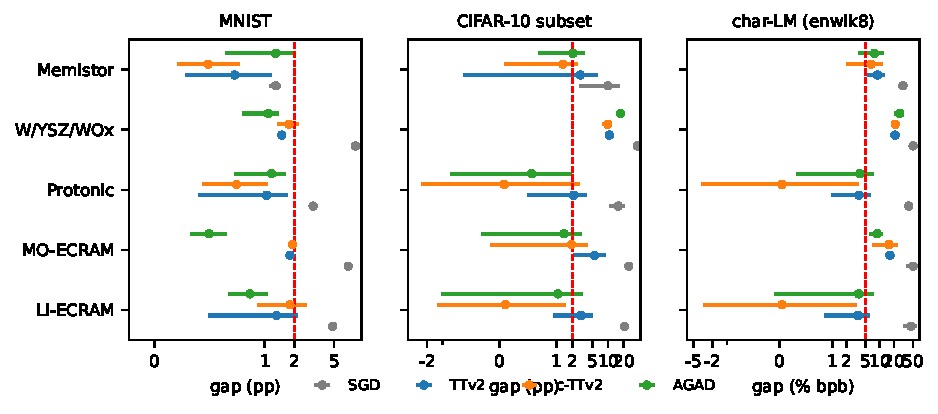
\includegraphics[width=\linewidth]{figs/fig_main}
\caption{Version 1 (superseded). Original simulator: gap to the exact-update baseline (mean and 95\% interval over 5 seeds; symmetric-log axis); the
dashed line is the gap line.}\label{fig:main}
\end{figure}
